% ---------------------
% DATASET ET FINE-TUNING DU MODELE DE DIFFUSION
% ---------------------
\chapter{Dataset et fine-tuning du modèle de diffusion} \label{ch_four}

\section{Justification du fine-tuning}

Les modèles SAM3, MoGe-2 et SAM 3D Body relèvent des architectures fondationnelles. Leur entraînement à très grande échelle leur permet une généralisation robuste ainsi qu'une spécialisation à la tâche de type \textit{zero-shot}, mais implique des contraintes en termes de ressources (voir section~\ref{sec:inference-sur-GPU}). À l'inverse, le modèle de complétion amodale vidéo par diffusion TACO dépend strictement de ses données d'apprentissage et il est mono-tache, il ne peut pas être utilisé directement pour la complétion amodale de sujets humains dans des vidéos de force athlétique sans adaptation préalable.

L'architecture TACO a été entraînée sur un dataset synthétique composé d'environ 200\,000 paires de vidéos~\cite{TACO-2025}, élaboré en superposant des occlusions artificielles sur des séquences sources préalablement identifiées comme non-occultées. Bien que cette méthode d'entraînement permette une adaptation sur des bases de données généralistes, son transfert direct vers l'analyse de la force athlétique expose certains problèmes :

\begin{itemize}
  \item \textbf{Manque d'occlusions spécifiques.} Le dataset OvO utilisé pour entraîner TACO~\cite{TACO-2025} est construit à partir de cinq sources génériques (MVImgNet, SA-V, BDD100K, SA-1B, Objaverse), couvrant des objets du quotidien, des scènes de conduite et des environnements intérieurs. Aucune de ces sources ne contient de séquences de force athlétique, et les auteurs ne décrivent aucune procédure de filtrage orientée vers ce domaine. La probabilité que des occlusions par des disques de fonte ou des racks à squat figurent dans le dataset d'entraînement est donc négligeable, ce qui justifie l'adaptation par fine-tuning.
  \item \textbf{Cadrages et perspectives atypiques.} Les vidéos issues d'environnements ouverts n'ont pas les mêmes angles de capture imposés par les standards d'évaluation de force athlétique (cadrage serré, prise de vue rasante).
\end{itemize}

L'incapacité des datasets publics à reproduire l'environnement de la force athlétique invalide l'usage direct du modèle. La création d'un dataset propriétaire, incluant les masques et les occlusions synthétiques spécifiques, ainsi qu'un \textit{fine-tuning} de TACO, constituent un prérequis pour garantir une restauration amodale correcte.

\section{Collecte et critères de sélection des vidéos}

Compte tenu de l'absence de dataset public adapté, une stratégie de collecte ciblée a été privilégiée à l'accumulation massive. Le dataset constitué comprend moins de 100 séquences vidéo (voir annexe~\ref{ann:dataset-details}), ce qui se justifie par l'adoption d'une stratégie de fine-tuning par adaptation à faible rang (LoRA, voir section~\ref{sec:protocole}) qui ne nécessite que peu de données pour spécialiser un modèle pré-entraîné.

\subsection{Sources de collecte}

Les vidéos sources ont été récoltées depuis deux canaux différents :

\begin{itemize}
  \item \textbf{Captations propres.} Une partie du dataset provient de sessions d'entraînement filmées par l'auteur de ce travail de fin d'études, dans des conditions contrôlées où le cadrage et le positionnement du matériel étaient maîtrisés (sujet seul dans le champ, équipement obstructif écarté lorsque l'exercice le permet).

  \item \textbf{Captations auprès de pratiquants volontaires.} La majorité du dataset provient de séquences filmées par des pratiquants de force athlétique sollicités spécifiquement pour ce mémoire. Chaque participant a filmé ses propres sessions d'entraînement selon certains paramètres fournis (cadrage, angle de prise de vue, conditions de captation).
\end{itemize}

Le recrutement de ces volontaires s'est avéré particulièrement long et restrictif, la communauté des pratiquants de force athlétique filmant leurs entraînements dans des conditions exploitables (caméra fixe, cadrage complet, qualité suffisante) reste limitée, et l'établissement tardif de la charte RGPD (voir annexe~\ref{ann:rgpd}) du projet (détaillant le consentement éclairé, la finalité de traitement, et les modalités de retrait) a réduit le temps disponible pour la collecte. Ce facteur explique en grande partie la taille restreinte du dataset constitué.

\subsection{Critères de sélection}

Les séquences retenues satisfont conjointement les critères suivants :

\begin{enumerate}
  \item \textbf{Visibilité intégrale du sujet.} L'athlète apparaît dans son entièreté dans le champ de vision (tête, tronc, membres supérieurs et inférieurs visibles), condition nécessaire pour disposer d'une référence non-occluse exploitable.
  \item \textbf{Absence d'occlusions au moment de la capture source.} La séquence ne contient pas d'éléments d'équipement masquant le sujet. Les occlusions seront ajoutées synthétiquement dans une seconde étape.
  \item \textbf{Stabilité du cadrage.} La caméra reste fixe ou présente des mouvements lents et continus, conformément à la pratique standard d'évaluation en force ahlétique.
  \item \textbf{Qualité visuelle suffisante.} Résolution minimale de 360p, fréquence de capture d'au moins 25 images par seconde, exposition correcte du sujet.
  \item \textbf{Diversité morphologique et vestimentaire.} Sélection veillant à représenter différents gabarits, sexes, tenues d'entraînement et types d'éclairage afin d'éviter un biais de spécialisation excessif.
  \item \textbf{Diversité des exercices.} Les trois mouvements de référence de la force athlétique sont représentés : squat, développé couché, soulevé de terre.
\end{enumerate}

\subsection{Axes de généralisation visés}

La constitution du dataset est guidée par cinq axes de variabilité selon lesquels le modèle fine-tuné doit généraliser, indépendamment du mouvement effectué :

\begin{itemize}
  \item \textbf{Variabilité inter-individu.} Morphologies, sexes et gabarits différents afin que le modèle ne mémorise pas une silhouette corporelle particulière.
  \item \textbf{Variabilité inter-éclairage.} Conditions lumineuses variées (éclairage artificiel de salle, lumière naturelle, contre-jour partiel) pour éviter une dépendance aux niveaux de luminosité ou aux températures de couleur spécifiques à un lieu.
  \item \textbf{Variabilité inter-salle.} Arrière-plans, textures de sol et configurations de salle différentes, afin que le modèle ne s'appuie pas sur des indices contextuels fixes pour la reconstruction.
  \item \textbf{Variabilité inter-caméra.} Résolutions, angles de capture et distances focales variées, reflétant la diversité des dispositifs utilisés par les pratiquants (smartphone, caméra, lentilles).
  \item \textbf{Variabilité inter-angle de prise de vue.} Les vidéos doivent être filmées depuis des angles variés (face, trois-quarts, profil) afin que le modèle ne soit pas biaisé vers une configuration de capture particulière. En compétition officielle, les caméras sont généralement positionnées de côté ou en trois-quarts, tandis que les entraînements sont fréquemment filmés de face. Couvrir ces différentes perspectives garantit une robustesse de la complétion amodale indépendamment de l'angle depuis lequel l'occlusion est observée.
  \item \textbf{Variabilité inter-matériel.} Disques, racks et bancs de marques et coloris différents, afin que la reconnaissance des occlusions synthétiques ne soit pas conditionnée à un équipement spécifique.
  \item \textbf{Variabilité inter-tenue.} Vêtements d'entraînement variés (couleurs, coupes, équipements de compétition tels que \textit{singlets} et genouillères) pour que la reconstruction de la silhouette soit robuste à la texture vestimentaire.
  \item \textbf{Variabilité du taux d'occlusion.} La surface du sujet masquée par l'occlusion varie selon le chargement de la barre (barre vide vs barre chargée avec plusieurs disques superposés), la phase du mouvement et l'angle de capture. Le dataset doit couvrir un spectre allant des occlusions partielles (un seul disque masquant une épaule) aux occlusions massives (barre chargée masquant intégralement le torse), afin que le modèle ne soit pas biaisé vers un taux d'occlusion particulier. Cette variabilité est partiellement contrôlée par la contrainte de couverture maximale de 60\,\% imposée lors de la génération synthétique des occlusions (voir section~\ref{sec:protocole}).
\end{itemize}

Ces axes de généralisation conditionnent directement la constitution des partitions du dataset. Idéalement, chaque partition devrait couvrir l'ensemble de ces axes de façon équilibrée, de sorte que la validation et le test mesurent effectivement la capacité de généralisation et non la mémorisation. En pratique, la taille restreinte du dataset (moins de 100 séquences) ne permet pas une couverture exhaustive et équilibrée de toutes les combinaisons. La partition est donc réalisée en veillant à ce qu'aucun individu, aucune salle et aucune configuration de matériel présents dans les données de tests ne figurent dans les données d'entraînements, minimisant ainsi le risque de surapprentissage sur les exemples vus.

\section{Stratégie d'annotation et construction des paires}

La construction du dataset de fine-tuning suit une procédure entièrement automatisée illustrée à la figure~\ref{fig:pipeline-finetuning}, qui réutilise les premiers modules du pipeline d'inférence décrits au chapitre~\ref{ch_three}. Cette réutilisation présente un avantage, les données d'entraînement présentent exactement la même distribution de prétraitement (segmentation, isolation du fond) que celles qui seront effectivement présentées au modèle en production, éliminant tout écart de domaine entre entraînement et inférence.

\begin{figure}
  [htp]
  \centering
  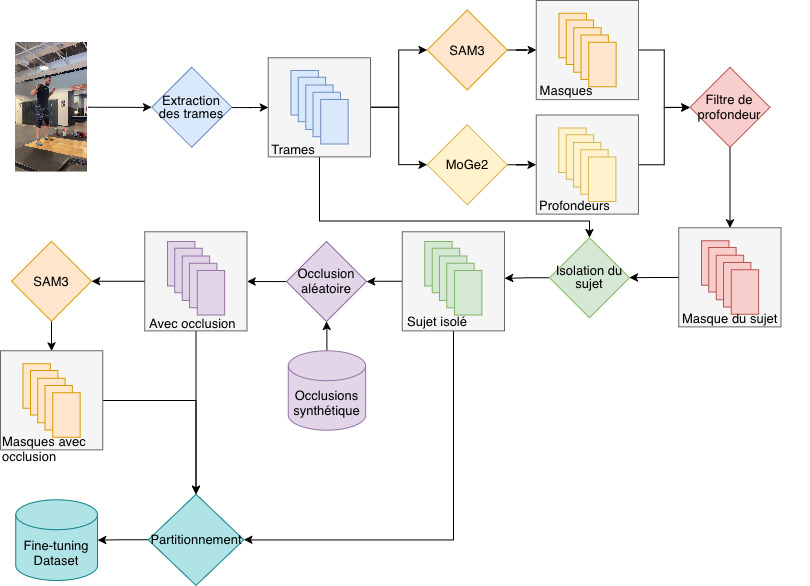
\includegraphics[height=9.5cm]{images/4-Dataset_and_fine-tuning/Dataset-Pipeline.jpg}
  \caption{Pipeline de construction du dataset de fine-tuning}
  \label{fig:pipeline-finetuning}
\end{figure}

\subsection{Extraction du sujet sur fond neutre}

Chaque séquence vidéo brute est d'abord traitée par les modules SAM3 et MoGe-2, suivis du filtre de profondeur. La sortie est l'ensemble des \emph{masques du sujet au premier plan} pour chaque trame de la séquence, identifiant l'athlète isolé du reste de la scène. Une étape de vérification manuelle est conduite trame par trame sur cette sortie. Cette vérification est essentielle sur un dataset de petite taille, chaque erreur d'annotation pèse proportionnellement plus lourd sur l'apprentissage.

L'étape suivante, dite d'\emph{isolation du sujet}, applique ce masque sur les images originales pour produire une séquence où seul l'athlète apparaît, le fond étant remplacé par du blanc uniforme. Ces images isolées constituent la cible (\emph{ground truth}) du fine-tuning, elles représentent la sortie idéale que le modèle TACO devrait produire face à des données occluses.

\subsection{Génération synthétique des éléments occultants}

À partir des images isolées, des occlusions synthétiques (figure~\ref{fig:occlusion-synthétique}) sont superposées aléatoirement. La stratégie reprend la méthodologie OvO (\emph{Object-video-Overlay}) introduite par les auteurs de TACO~\cite{TACO-2025}, mais avec une banque d'occlusions synthétiques spécialisée pour la force athlétique :

\begin{itemize}
  \item \textbf{Disques de fonte calibrés.} Banque d'images de disques de compétition provenant du catalogue produit du distributeur Rogue Fitness~\cite{Rogue-Fitness-Plates}, extraits sur fond transparent depuis des photographies à haute résolution. Les disques respectent le code couleur normalisé par l'IPF \footnote{L'\textit{International Powerlifting Federation} (IPF) impose un code couleur strict pour les disques de compétition~\cite{IPF-Technical-Regulations-2025} : rouge pour 25\,kg, bleu pour 20\,kg, jaune pour 15\,kg, vert pour 10\,kg et blanc pour 5\,kg. Ce code couleur universel garantit l'identification rapide des charges par les juges et les athlètes lors des compétitions officielles.} (5, 10, 15, 20 et 25\,kg). Des images de disques provenant de salles commerciales, dont les couleurs peuvent différer des standards IPF, ont également été intégrées à la banque afin d'améliorer la diversité visuelle. Un retournement horizontal (\textit{flip}) a été appliqué à chaque occlusion pour doubler la diversité des configurations. Des configurations à disques multiples ont également été générées en superposant plusieurs disques de diamètres différents, reproduisant l'apparence d'une barre chargée à l'entrainement où plusieurs disques sont empilés de part et d'autre de l'axe.
  \item \textbf{Racks à squat.} Banque d'images de structures verticales et horizontales (montants de rack et sécurités) également extraites sur fond transparent. Ces éléments reproduisent l'obstruction caractéristique observée lors des squats où les montants du rack masquent partiellement le torse ou les jambes du sujet.
\end{itemize}

Pour chaque clip isolé, une occlusion est sélectionnée aléatoirement dans la banque. Pour chaque occlusion, une position aléatoire est calculée permettant à l'occlusion de masquer une partie visible du sujet.


\begin{figure}
  [htp]
  \centering
  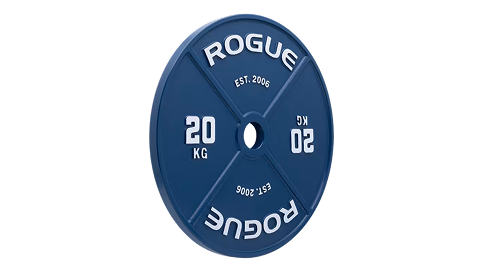
\includegraphics[width=4.5cm, height=2.5cm]{images/4-Dataset_and_fine-tuning/object_13_plate.png}
  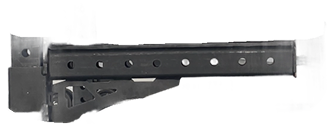
\includegraphics[width=4.5cm, height=2.5cm]{images/4-Dataset_and_fine-tuning/object_10_rack.png}
  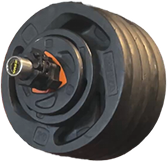
\includegraphics[width=2.5cm, height=2.5cm]{images/4-Dataset_and_fine-tuning/object_3_plate.png}
  \caption{Illustration de 3 exemples d'occlusions synthétiques}
  \label{fig:occlusion-synthétique}
\end{figure}

\subsection{Recalcul du masque visible}

Une fois la version occluse obtenue, une seconde passe de SAM3 est effectuée sur ces images pour produire le \emph{masque du sujet avec occlusion}, c'est-à-dire le masque ne couvrant que les portions visibles du sujet après superposition. Ce recalcul par SAM3 est préféré à un simple calcul de différence pour deux raisons :

\begin{itemize}
  \item \textbf{Robustesse aux occlusions synthétiques à contours flous.} Les bords d'un disque avec une transparence partielle ne sont pas binaires, SAM3 produit un masque visible cohérent avec ce qui est effectivement perçu, là où une différence produirait des contours aberrants.
  \item \textbf{Cohérence avec le pipeline d'inférence.} En réalité, le masque visible du sujet sera effectivement calculé par SAM3 sur les images occluses. Reproduire cette même procédure lors de la construction du dataset garantit que TACO est entraîné dans les mêmes conditions qu'il sera utilisé.
\end{itemize}

Le triplet (\texttt{occluded\_frame}, \texttt{visible\_mask}, \texttt{amodal\_object}) constitue un échantillon d'entraînement : les deux premiers éléments forment l'entrée fournie au modèle (la trame occluse à reconstruire et le masque indiquant les régions visibles du sujet), le troisième la cible (le sujet isolé non occlus servant de vérité terrain).

Le dataset complet est partitionné en sous-ensembles d'entraînement (70\,\%, 17 vidéos sources, 136 séquences) et de validation (30\,\%, 6 vidéos sources, 48 séquences) selon un découpage aléatoire par vidéo source (graine fixée à 42), garantissant que toutes les augmentations dérivées d'une même vidéo source (\textit{original}, \textit{blur}, \textit{contrast}, \textit{flipped}, etc.) sont systématiquement assignées à la même partition. Ce choix prévient toute fuite de données liée à la présence simultanée de variantes quasi-identiques en entraînement et en évaluation.

Cependant, le découpage étant réalisé par vidéo et non par sujet, quatre sujets apparaissent simultanément dans les partitions d'entraînement et de validation. Cette situation représente une limite méthodologique car la validation mesure partiellement la capacité du modèle à généraliser à de nouveaux individus et sa capacité à généraliser à de nouvelles sessions d'un même individu. Un découpage strict par sujet aurait été préférable mais n'était pas réalisable compte tenu du nombre limité de sujets distincts disponibles dans le dataset.

\subsection{Adaptation des dimensions au format d'entrée du modèle}

Les trames extraites des vidéos sources sont initialement de dimensions variables (typiquement 1920$\times$1080 ou 1280$\times$720 selon les vidéos). Le modèle TACO requiert des entrées au format $384 \times 384$, correspondant à la résolution native d'entraînement du checkpoint et au compromis le plus stable en mémoire sur la configuration matérielle disponible (2$\times$RTX A5000 de 24 Go).

Le chargeur de données (\textit{dataloader}) natif de TACO (\texttt{VACDataset}) applique un redimensionnement direct vers $384 \times 384$ au chargement de chaque trame, sans préservation du ratio d'aspect. Cette stratégie, choisie par les auteurs du modèle pour homogénéiser le format d'entrée, introduit une déformation du sujet, une trame $16:9$ source se voit comprimée verticalement (ou étirée horizontalement) pour s'inscrire dans un format carré.

Deux conséquences méthodologiques en découlent :

\begin{itemize}
  \item \textbf{Cohérence entrainement/inférence.} L'entraînement et l'inférence appliquent la même déformation, donc le modèle apprend à reconstruire des silhouettes anatomiquement déformées mais cohérentes avec ce qui sera présenté en production. Tant que le pipeline finale applique le même prétraitement, les proportions seront restituées correctement à la sortie.
  \item \textbf{Anatomie apprise déformée.} Le modèle apprend des proportions corporelles distordues par le ratio. Pour une utilisation impliquant des mesures biomécaniques précises (angles articulaires), il sera nécessaire d'appliquer une transformation inverse en post-traitement ou d'envisager un crop préalable préservant le ratio. Il a été choisi de faire une transformation inverse en post-traitement pour récupérer les proportions anatomiques de départ, afin de ne pas introduire de nouveaux artefacts liés à un recadrage (perte d'information sur les extrémités, variations de cadrage entre les vidéos sources) et pour conserver la simplicité du pipeline d'entraînement.
\end{itemize}

\section{Augmentation et équilibrage du dataset}

Pour pallier la taille restreinte du dataset (moins de 100 séquences), des stratégies d'augmentation de données ont été utilisées.

\subsection{Augmentation par variation des occlusions synthétiques}

Une banque d'occlusions synthétiques a été constituée, regroupant deux catégories distinctes :
\begin{itemize}
  \item \textbf{Disques} : configurations variant selon le nombre de disques superposés sur la barre et leur couleur, correspondant aux différents poids selon les standards IPF (5, 10, 15, 20, 25\,kg), chaque couleur étant associée à un calibre spécifique.
  \item \textbf{Racks} : structures de support fixes utilisées comme sécurité lors du mouvement de squat.
\end{itemize}

Pour chaque clip d'entraînement, une occlusion unique est tirée aléatoirement dans la banque et conservée pendant toute la durée de la séquence, afin de simuler une occlusion temporellement cohérente. Le comportement spatial de l'occlusion dépend de sa catégorie. Les racks sont positionnés à un emplacement fixe à proximité du sujet, reproduisant le caractère statique de ce type d'élément dans la scène réelle. Les disques suivent une trajectoire verticale montante ou descendante au fil des trames, leur position horizontale restant constante. Le déplacement du disque reproduisant la dynamique d'une barre en mouvement durant un mouvement.

La position initiale, le calibre et l'amplitude de la trajectoire sont rééchantillonnés à chaque itération, sous la contrainte que la couverture de la silhouette n'excède jamais 60\,\% sur les trames du clip. Cette stratégie multiplie considérablement la diversité des configurations vues par le modèle, combinée aux 8 augmentations visuelles par vidéo source et à l'échantillonnage temporel aléatoire effectué par le dataloader (voir la section~\ref{sec:protocole}), elle permet de générer plusieurs milliers de paires d'entraînement distinctes au cours des 100 époques, là où un dataset statique se limiterait à un nombre fixé de paires figées.

\subsection{Augmentation visuelle standard}

Des transformations visuelles classiques sont appliquées de façon synchronisée sur l'ensemble du clip:

\begin{itemize}
  \item Variation colorimétrique (luminosité, contraste, saturation).
  \item Miroir horizontal.
  \item Légère rotation aléatoire des vidéos (max +- 10°).
\end{itemize}

Les transformations géométriques agressives (perspective, déformations, ...) sont volontairement exclues car elles altèrent l'anatomie du sujet et entreraient en conflit avec l'apprentissage de la complétion amodale anatomiquement plausible.

\subsubsection{Échantillonnage temporel aléatoire}

À chaque itération d'entraînement, le dataloader sélectionne aléatoirement une fenêtre temporelle de 14 trames consécutives parmi les trames disponibles dans chaque séquence. La graine aléatoire est fixée à 1234, garantissant la reproductibilité de l'échantillonnage entre deux exécutions identiques. Cette stratégie, héritée du protocole d'entraînement original de TACO~\cite{TACO-2025}, présente un double bénéfice :

\begin{itemize}
  \item Elle multiplie le nombre de clips uniques visibles par le modèle, agissant comme une augmentation temporelle.
  \item Elle expose le modèle à toutes les phases du mouvement (initiale, concentrique, statique, excentrique) plutôt qu'à un timing fixe, améliorant la généralisation à des séquences de test pouvant débuter à n'importe quel instant du cycle d'exercice.
\end{itemize}

Sur l'ensemble de l'entraînement, le modèle est ainsi exposé à une grande diversité de configurations temporelles, sans surcoût mémoire et sans modification du dataset.

\section{Protocole d'entraînement et hyperparamètres}
\label{sec:protocole}

\subsection{Choix du fine-tuning par LoRA}

Le fine-tuning complet de TACO est techniquement infaisable dans ce contexte ci, le modèle qui est basé sur Stable Video Diffusion, comporte de l'ordre de 2,4 milliards de paramètres, et son entraînement complet requerrait plusieurs dizaines de Go de VRAM, soit bien au-delà des 48 Go disponibles (2 $\times$ 24 Go) sur la machine mise à disposition. De plus, un fine-tuning complet sur un dataset de moins de 100 vidéos sources entraînerait un sur-apprentissage massif et une dégradation des capacités généralistes du modèle pré-entraîné~\cite{LoRA-2021}.

La stratégie retenue est donc le fine-tuning par adaptation à faible rang (\emph{Low-Rank Adaptation}, LoRA)~\cite{LoRA-2021}. 

Cette paramétrisation présente deux avantages dans ce contexte. D'une part, les gradients et les états de l'optimiseur ne sont calculés et stockés que pour les 11,7 millions de paramètres entraînables, contre 2,4 milliards pour un fine-tuning complet, réduisant drastiquement l'empreinte mémoire GPU liée à l'optimisation et rendant l'entraînement réalisable sur deux RTX A5000. D'autre part, la contrainte de faible rang limite la capacité d'adaptation du modèle, ce qui est souhaitable sur un dataset de petite taille où un fine-tuning complet conduirait inévitablement au sur-apprentissage~\cite{LoRA-2021}.

\subsection{Configuration LoRA}

La stratégie d'adaptation à faible rang utilisée est celle implémentée nativement dans le code source de TACO sous l'identifiant \texttt{ft\_strategy: time\_lora}~\cite{TACO-2025}. Cette stratégie présente deux caractéristiques importantes :

\begin{itemize}
  \item \textbf{Ciblage des couches temporelles uniquement.} La stratégie \texttt{time\_lora} ajoute des adaptateurs LoRA exclusivement sur les modules linéaires associés au traitement temporel. Les modules d'attention spatiale, quant à eux, sont intégralement gelés (\textit{frozen}) : leurs paramètres originaux ne reçoivent aucun gradient et aucun adaptateur LoRA ne leur est associé.

  \item \textbf{Cohérence avec le domaine d'adaptation.} Ce ciblage temporel correspond à la nature de l'adaptation souhaitée, ce qui distingue la force athlétique des séquences génériques du dataset OvO original n'est pas l'apparence du sujet mais la dynamique temporelle des occlusions synthétiques, avec des trajectoires verticales caractéristiques de la barre pendant les phases concentriques et excentriques. Limiter l'adaptation aux modules temporels réduit ainsi le risque de \emph{catastrophic forgetting} \footnote{Le \textit{catastrophic forgetting} désigne le phénomène par lequel un réseau de neurones, lors d'un apprentissage sur de nouvelles données, dégrade rapidement et irrémédiablement les connaissances acquises lors d'un entraînement précédent. Ce phénomène est particulièrement problématique lors du fine-tuning de modèles fondationnels sur des datasets spécialisés de petite taille, où le risque de surspécialisation au détriment des capacités générales est élevé.~\cite{catastrophic-forgetting-2015}} sur les capacités spatiales du modèle pré-entraîné.
\end{itemize}

Le rang LoRA est fixé à $r=16$ par l'implémentation de référence. Ce paramètre $r$ contrôle la dimension des matrices de faible rang \footnote{Une matrice de faible rang est une matrice dont le rang (c'est-à-dire le nombre de dimensions indépendantes de son espace colonne) est très inférieur à ses dimensions. En pratique, une matrice $\Delta W \in \mathbb{R}^{d \times d}$ de rang $r \ll d$ peut être approximée par le produit de deux matrices rectangulaires plus petites, réduisant drastiquement le nombre de paramètres nécessaires pour la représenter. LoRA exploite cette propriété pour paramétrer les mises à jour des poids du modèle de manière compacte, sans modifier les poids originaux.} introduites par LoRA : plus $r$ est petit, moins le modèle dispose de capacité d'adaptation, mais plus il est résistant au sur-apprentissage.

Avec $r=16$, la stratégie \texttt{time\_lora} aboutit à 11{,}7 millions de paramètres entraînables sur les 2,4 milliards de paramètres totaux du modèle, soit environ 0{,}49\,\% du total.

\subsection{Hyperparamètres d'entraînement}

Le protocole d'entraînement reprend la configuration de référence de TACO~\cite{TACO-2025} pour les composants hérités du modèle pré-entraîné (par exemple : \textit{sampler}, \textit{loss}, \textit{encodeur}) et y adapte les paramètres de parallélisation et de durée pour la configuration matérielle disponible. La configuration originale des auteurs requiert un système à 8 GPU NVIDIA H100 de 80 Go chacune (soit 640 Go de VRAM au total). Le matériel utilisé dans ce mémoire (2 GPU NVIDIA RTX A5000 de 24 Go, soit 48 Go au total) impose plusieurs adaptations détaillées dans le tableau~\ref{tab:hyperparams}.

\begin{table}[h]
  \centering
  \begin{tabular}{ll}
    \hline
    \textbf{Paramètre} & \textbf{Valeur} \\
    \hline
    \multicolumn{2}{l}{\textbf{Configuration de TACO}} \\
    Optimiseur & Adam* \\
    Taux d'apprentissage de base & $2 \times 10^{-5}$* \\
    Résolution des trames & $384 \times 384$* \\
    Nombre de trames par clip & 14* \\
    Sampler de diffusion & EulerEDMSampler, 25 pas* \\
    Discrétisation & EDM, $\sigma_{\max} = 700$* \\
    Guidage & LinearPredictionGuider, échelle 1{,}0--2{,}5* \\
    Loss & StandardDiffusionLoss + EDMWeighting* \\
    Échantillonnage des sigmas & EDM, $p_{\text{mean}} = 1{,}0$, $p_{\text{std}} = 1{,}6$* \\
    Augmentation du conditionnement & $0{,}02$* \\
    Probabilité d'inversion temporelle & $0{,}2$* \\
    Gradient checkpointing & activé (\texttt{use\_checkpoint: True})* \\
    Stratégie LoRA & \texttt{ft\_strategy: time\_lora}* \\
    Checkpointing & toutes les 1\,000 itérations* \\
    \hline
    \multicolumn{2}{l}{\textbf{Paramètres LoRA}} \\
    Rang LoRA $r$ & 16 (hardcodé dans l'implémentation) \\
    Couches ciblées & Attentions temporelles, feed-forward et embeddings temporels \\
    Couches non adaptées & Attentions spatiales, VAE, embeddings de \\
    & conditionnement (CLIP) \\
    Paramètres entraînables & 11{,}7\,M / 2{,}4\,B ($\approx 0{,}49\,\%$) \\
    \hline
    \multicolumn{2}{l}{\textbf{Paramètres adaptés à la configuration}} \\
    Graine aléatoire (\textit{seed}) & 1234 \\
    Stratégie multi-GPU & DDP (Distributed Data Parallel) \\
    Batch size par GPU & 1 (au lieu de 2 dans la configuration originale) \\
    Accumulation de gradient & $\times 2$ \\
    Batch effectif total & 4 ($1 \times 2$ GPU $\times 2$) \\
    Précision & mixte 16-bit (AMP) \\
    Nombre d'époques maximales & 100 (au lieu de 300) \\
    \hline
  \end{tabular}
  \caption{Hyperparamètres du fine-tuning LoRA de TACO. Les valeurs marquées d'un astérisque correspondent à la configuration de référence des auteurs.}
  \label{tab:hyperparams}
\end{table}

Trois adaptations notables sont apportées par rapport à la configuration de référence des auteurs. Premièrement, les ressources matérielles disponibles (2$\times$RTX A5000, 24\,Go chacune) sont très inférieures à la configuration originale (8$\times$H100, 80\,Go chacune). Cette contrainte mémoire impose de réduire le batch size \footnote{Le (\textit{batch size}) correspond au nombre d'exemples d'entraînement traités simultanément par itération.} par GPU à 1 clip, là où les auteurs en utilisaient 2. Pour compenser partiellement cette réduction sans modifier la dynamique d'optimisation, une accumulation de gradient sur 2 pas est appliquée : le gradient est calculé sur 2 clips successifs avant chaque mise à jour des poids, ce qui produit un batch effectif de $1 \times 2\,\text{GPU} \times 2\,\text{accumulations} = 4$ clips par mise à jour. Cette valeur reste inférieure au batch effectif de la configuration originale ($2 \times 8\,\text{GPU} = 16$ clips), mais constitue le maximum réalisable sur le matériel disponible. Cette différence implique que les mises à jour des poids sont calculées sur un gradient plus bruité, ce qui peut ralentir légèrement la convergence mais ne compromet pas la validité de l'entraînement, d'autant que la taille réduite du dataset limite de toute façon le nombre d'itérations nécessaires. Deuxièmement, le nombre maximal d'époques est ramené de 300 à 100. Le dataset spécialisé compte 136 séquences d'entraînement (17 vidéos sources $\times$ 8 augmentations visuelles) et 48 séquences de validation (6 vidéos sources $\times$ 8 augmentations). À chaque itération, le chargeur de données sélectionne aléatoirement un \texttt{frame\_start} $\in [0, N - 14]$ où $N$ est le nombre total de trames de la séquence, puis extrait les 14 trames consécutives à partir de cet indice. Cette stratégie expose le modèle à toutes les phases du mouvement (descente, point de retournement, remontée) au fil des époques, sans nécessiter de découpage préalable des séquences en clips fixes. C'est en effet bien inférieur en taille au dataset OvO original, ce qui réduit mécaniquement le nombre d'itérations nécessaires pour couvrir l'ensemble des données. De plus, la convergence par adaptation LoRA est généralement plus rapide que le pré-entraînement complet, le modèle partant d'un état déjà initialisé~\cite{LoRA-2021}. Troisièmement, le taux d'apprentissage de base ($2 \times 10^{-5}$) est conservé pour les adaptateurs LoRA. Ce choix est motivé par la cohérence avec le pré-entraînement : utiliser un taux d'apprentissage plus élevé risquerait de déstabiliser les représentations apprises, tandis qu'un taux plus faible ralentirait inutilement la convergence sur un dataset de petite taille.

La parallélisation DDP \footnote{\textit{Distributed Data Parallel} (DDP)~\cite{Li-DDP-2020}  est une stratégie d'entraînement multi-GPU dans laquelle chaque GPU dispose d'une copie complète du modèle et traite un sous-ensemble distinct des données. Les gradients calculés sur chaque GPU sont synchronisés et moyennés à chaque pas de mise à jour, garantissant que tous les GPU maintiennent des poids identiques. Cette approche présente une efficacité quasi-linéaire avec le nombre de GPU, contrairement au parallélisme de modèle où le modèle est découpé entre les GPU.} entre les deux GPU A5000 permet de diviser le temps d'entraînement par un facteur proche de 2 par rapport à une exécution mono-GPU, sans compromettre la convergence.

\subsection{Fusion des adaptateurs LoRA.}

À l'issue de l'entraînement, les adaptateurs LoRA (voir annexe~\ref{ann:lora-config}) sont fusionnés dans les poids du modèle de base via un script dédié. Pour chaque couche ciblée, la mise à jour $\Delta W = \frac{\alpha}{r} B \times A$ est additionnée aux poids originaux $W$, produisant un checkpoint unique utilisable directement par TACO en inférence, sans dépendance à la bibliothèque PEFT et sans surcoût computationnel par rapport au modèle baseline.

\subsection{Stratégie de validation et de sélection de modèle}

Le dataset est divisé en deux partitions : 70\,\% entraînement (17 vidéos sources, 136 séquences), 30\,\% validation (6 vidéos sources, 48 séquences), avec un découpage par séquence source (et non par clip) pour éviter toute fuite de données entre partitions. Les vidéos contenant des occlusions réelles sont exclues des deux partitions. La validation est conduite à chaque époque sur l'ensemble de la partition de validation (48 séquences), l'entraînement lui est conduit sur un maximum de 100 époques. Le modèle sélectionné est celui correspondant à la 100e époque.

\section{Évaluation qualitative et quantitative}

\subsection{Métriques quantitatives}

Deux métriques complémentaires sont utilisées pour évaluer la qualité de la complétion amodale sur le jeu de données de test, calculées entre la vidéo reconstruite et la vidéo de référence :

\begin{itemize}
  \item \textbf{SSIM} (\textit{Structural Similarity Index})~\cite{SSIM-2004}. Évalue la similarité structurelle locale entre images, plus robuste que le PSNR (\textit{Peak Signal-to-Noise Ratio} \footnote{Mesure pixel-à-pixel exprimée en décibels, sensible à la fidélité géométrique et colorimétrique. Calculée uniquement sur les régions occluses puis moyennée sur toutes les trames du clip}) aux changements d'éclairage ou de contraste. Calculée par fenêtres glissantes puis moyennée sur les régions occluses.
  
  \item \textbf{LPIPS} (\textit{Learned Perceptual Image Patch Similarity})~\cite{LPIPS-2018}. Métrique reconnue pour mieux corréler avec le jugement humain que les métriques pixel-à-pixel. Particulièrement pertinente dans notre cas, où la fidélité plausible du corps reconstruit importe davantage que la fidélité pixel-exacte.
\end{itemize}

Les deux métriques sont rapportées avant et après fine-tuning, sur le modèle TACO pré-entraîné par les auteurs et sur notre modèle fine-tuné. Une amélioration significative sur LPIPS combinée à une stabilité ou amélioration sur SSIM constitue le critère de succès du fine-tuning. L'impact de cette amélioration sur la reconstruction 3D est évalué séparément en section~\ref{sec:implications-pipeline} via le MPJPE (\textit{Mean Per-Joint Position Error})\footnote{Le MPJPE est la métrique standard pour évaluer la qualité d'une reconstruction de pose 3D. Pour chaque trame, il calcule la distance euclidienne moyenne entre les positions 3D prédites et les positions 3D de référence pour l'ensemble des articulations du squelette, exprimée en millimètres. Une valeur faible indique une reconstruction fidèle à la vérité terrain.} calculé sur les sorties de SAM 3D Body.

\subsection{Évaluation qualitative}

L'évaluation quantitative étant insuffisante pour caractériser la qualité d'une reconstruction générative, une inspection qualitative est conduite sur l'ensemble du jeu de données de test. Pour chaque clip, sont visualisées en juxtaposition :

\begin{itemize}
  \item la vidéo originale
  \item la vidéo occluse
  \item la complétion amodale par TACO baseline
  \item la complétion amodale par TACO fine-tuné
\end{itemize}

L'analyse porte sur la cohérence anatomique (proportion des différentes parties du corps, position des articulations, ...), la cohérence temporelle (absence de scintillement entre trames consécutives), et le réalisme textural (continuité de l'habillement, couleur de peau, ...).


\medskip
Le chapitre suivant présente les résultats expérimentaux obtenus à l'issue de l'entraînement, et les comparent avec les performances du modèle baseline.